\documentclass[12pt, border=5mm]{article}
\usepackage{amsmath}
\usepackage{tikz}
\begin{document}

\title{Jumlah Sudut Dalam Segitiga}
\author{Course and Tutor Course}
\maketitle

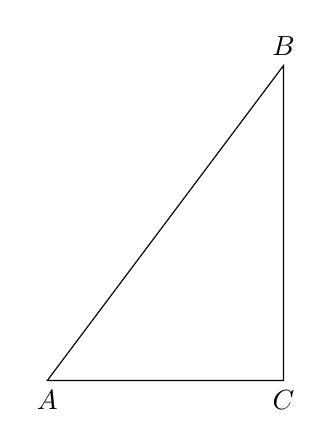
\begin{tikzpicture}
\draw (0,0) node[anchor=north]{$A$}
-- (3,0) node[anchor=north]{$C$}
-- (3,4) node[anchor=south]{$B$}
-- cycle;
\end{tikzpicture}

Besar sudut B dalam segitiga di atas adalah...\newline
Jumlah semua sudut pada segitiga adalah $180^{0}$ maka diperoleh:

$$
\begin{aligned}
&\angle{A}+\angle{B}+\angle{C} & = & 180^{0} \\
&60^{0}+90^{0}+30^{0} & = & 180^{0} \\
&150^{0}+30^{0}
\end{aligned}
$$
\end{document}
